\documentclass[12pt]{article}
\usepackage{amsmath,amssymb,bookmark,graphicx,parskip,custom}
\usepackage[margin=.8in]{geometry}
\allowdisplaybreaks
\hypersetup{colorlinks,
    citecolor=black,
    filecolor=black,
    linkcolor=black,
    urlcolor=black
}
\setcounter{secnumdepth}{5}

\begin{document}

\title{Git}
\author{Kevin Carruthers, Lara Janecka, Nik Klassen, Eric Pemberton}
\date{\vspace{-2ex}Fall 2015}
\maketitle\HRule

\tableofcontents
\newpage

\section{System Functionality}
Git is a version control system (VCS) designed to provide a powerful, distributed system for tracking file changes.

\begin{itemize}
\item As a software developer, I want to have a distributed workflow so that I can work offline and not have to connect to the main repository.
\item As a server administrator,  I want my repository to stay safe from content corruption so that I can be assured of the integrity of my data.
\item As a software developer, I want the system to have high performance so that this system does not interfere with my workflow.
\item As a software engineer, I want version control to integrate with my existing tools so that I have a seamless environment.
\item As a quality assurance manager, I want to be able to see the changes that have been made to the codebase so that I can ensure that appropriate testing has been done.
\item As a team member, I want to be able to work independently from the main code and then merge my changes into the main codebase, so that I can focus solely on the changes I’m making.
\end{itemize}

\section{Quality Attributes and Scenarios}
\subsection{Usability}
The system should behave in a way that is consistent with other version control systems that developers have experience with.

\begin{itemize}
\item Most developers using git work with a Unix-like operating system. Git will be most usable to them if it has an easily scriptable interface so that it can be integrated into their scripts.
\item There are lots of different operations that a version control system can do. A developer should be able to understand how these commands relate to each other so that they can intuitively know what effect the command they are using will have.
\end{itemize}

\subsection{Reliability}
The system must have very high reliability, failing far less than 1\% of the time.

\begin{itemize}
\item Git must be able to handle any number of developers pushing changes to the server at the same time, without corrupting data.
\end{itemize}

\subsection{Performance}
The system must be able to perform common operations in less than a couple seconds.

\begin{itemize}
\item A developer creates and checks out a branch. This process should take less than 5 seconds
\item The git log command should immediately show at least the last 10 commit messages to the user.
\end{itemize}

\section{Architectural Views}
\subsection{File Structure}
\begin{figure}[htbp]
\centering
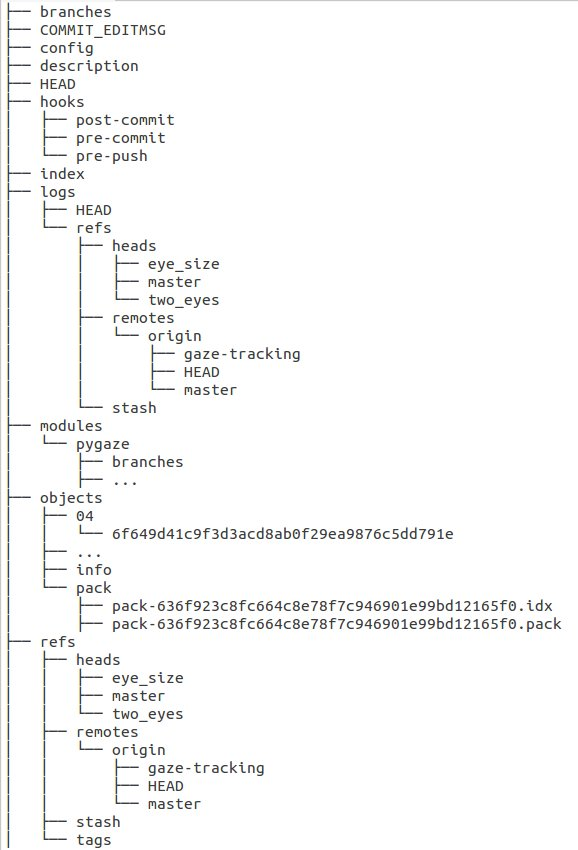
\includegraphics[width=0.5\textwidth]{filestructure.jpeg}
\caption{File structure of .git folder}
\label{fig:file}
\end{figure}

Figure~\ref{fig:file} displays the file structure of the .git folder for one group members SE390 internal miniproject. The git file structure is broken up into numerous sub folders used to manipulate the git tree.

\begin{description}
\item[The branches folder] contains information needed to manage branches (this is deprecated so the folder is empty).
\item[The COMMIT\_EDITMSG] file stores the last commit message.
\item[The config folder] contains the git configuration specific to this project. This example did not have any project specific configurations so the folder is empty.
\item[The description folder] is empty because it is used to contain information necessary for viewing the repository through a web client -- this was not used for this project.
\item[The HEAD file] stores a reference to which branch you are currently on, and
\item[The hooks folder] contains scripts to be executed on triggers defined by its subfolders post-commit, pre-commit, and pre-push.
\item[The index] contains information of what changes have been ``added'' and will be committed when the user runs the commit command.
\item[The logs folder] contains all changes that have been made in the history of the repository.
\item[The modules folder] outlines submodules that were included. In the example given it is seen as the pygaze module which contains the .git folder for that module so that git knows how to interact with it.
\item[The objects folder] stores all git objects (the hierarchy of these can be seen in Figure~\ref{fig:objects}) referenced by their SHA.
\item[The refs folder] contains references to all local heads (corresponding to all local branches) and all remote heads (corresponding to all remote branches).
\end{description}

Note that the index and logs folders do not contain the same data: the index only contains information that has been added and not committed.

The history of the git repository is stored by reference which are heads (referring to the heads of branches the names of which are the subfolders) or remotes (referring to branches that have been pushed).

\subsection{Object Structure}
\begin{figure}[htbp]
\centering
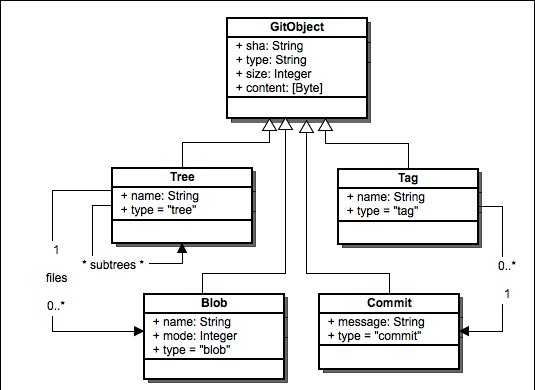
\includegraphics[width=0.75\textwidth]{objects.jpeg}
\caption{Object hierarchy for git}
\label{fig:objects}
\end{figure}

Git manages repositories through a tree of git objects. The UML for this is in Figure~\ref{fig:objects}. All objects are contain a large string called its sha through which you can reference that object. All content in a repository is stored in Blob objects and ordered into a tree objects. Each Blob represents a file stored in memory. The tree structure represents a directory. Commit objects point at the tree representing the top level directory of the commit. Tags are objects pointing to a single commit for use by the repository history.

\section{Architectural Analysis}
In order to create a usable program that is familiar to most users, git built its architecture with a toolkit design philosophy that is divided into two main parts; the plumbing and the porcelain. This follows the pattern of traditional Unix command line tools where the plumbing consists of low-level commands used to enable basic content tracking and the porcelain is a smaller subset of git commands that most users are likely to use in order to maintain, update and interact with their repositories. Git has a tree of commands and implements a call return pattern to execute commands. When a user executes a command a call propagates up the tree to any other commands that may need to be run as part of the original call. The command executes any work that is required of it and the final result is then returned back down the tree.

Another large design decision when building any VCS is how the system should store content. Subversion, an older VCS stored content in a delta-based changeset but Git chose to diverge from this instead using DAGs (Directed Acyclic Graphs). This means that instead of flattening the content and storing the change sets Git is instead able to create an object hierarchy of change data mirroring the filesystem tree as a snapshot of the user’s commit. DAG’s are also used to store Git’s commit and merge histories. Each node contains metadata about its ancestors. This method grants git full branching capabilities and merging 2 branches is the equivalent of merging nodes within the DAG (see Figure~\ref{fig:dag}).

\begin{figure}[htbp]
\centering
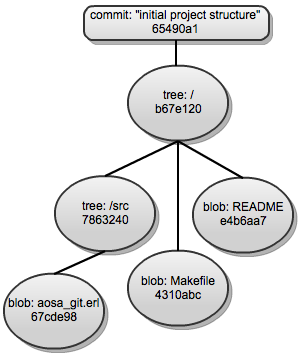
\includegraphics[width=0.5\textwidth]{dag.png}
\caption{Git DAG example}
\label{fig:dag}
\end{figure}

To be performant, git tackles the storage space problem by storing files in a compressed format with an index file that points to specific objects in that file. In addition, git keeps track of changes in each file rather than the files themselves by creating ``diff'' objects which show the differences between revisions. If there are only 2 changes in 10 commits, only 2 diffs of that file are stored (unlike the Subversion implementation which stores a full copy of the file for each change). This makes creating a branch much easier because only new diffs need to be stored instead of copying the entire project (Subversion). Git also increases speed and decreases latency through design decisions that were made. As an example, ``git log'' immediately returns the first page of results while it continues to generate the full history in the background. When fetching new changes, git checks which objects exist locally and only sends compressed differences in the form of a thin packfile. Git also does some operations locally instead of over the network. A network call is needed to get logs or compare the current working area to a different version in Subversion, but in git it is done locally

Git is built for version control and is trusted by large software projects to reliably store the history and project data.Internally, there are a lot of internal tools to help users to view the status of and maintain their repositories. Due to its tree structure and commit data it is able to track commits and place them in the appropriate place in the commit tree. It is even capable of handling multiple commits simultaneously by applying them on top of each other and returning merge conflicts if there is an issue instead of corrupting the data.

\section{Key Weaknesses}
Since git is written as a nested script-based architecture, it is not designed to be library-first; that is, the git implementation is designed to be executed as-is rather than imported into other tools. This can cause problems in the cases of, for example, IDEs, which thus can not simply import the specific submodule they desire but must instead execute the script as a forked process. This could be fixed by designing git as a library-first application and simply calling the various module entry-points from a shell script (in order to maintain the current interface).

Additionally, since the git modules are designed in the tree-based fashion outlined above, the architecture may be difficult for new users to comprehend. When they are searching for the method to perform some task, new users must try each submodule until they find the correct one. This could be addressed by merging similar submodules in order to try to make the system simpler, though this may have the side-effect of creating a system which is less powerful and customizable to more advanced users.

\section{References}
\begin{itemize}
\item Git Tutorial: Directory Structure - https://www.siteground.com/tutorials/git/directory.htm
\item The Architecture of Open Source Applications - http://aosabook.org/en/git.html
\end{itemize}

\end{document}
